\documentclass[../main.tex]{subfiles}
\begin{document}
\subparagraph{Problem 1}\label{subpar:problem1_rom}

Since we stored only the time-asymptotic (stable) equilibria of \eqref{eq:heat}, the snapshot matrix $\boldsymbol{X}$ is time-independent.
This means that our ansatz \eqref{eq:ansatz} for the ROM reduces to

\begin{equation*}
        \Pi_{\mathcal{R}_{h}}\boldsymbol{u}_{h}=\sum_{j=1}^{N_{r}}\bar{u}_{j}(t,\mu)\boldsymbol{v}_{j}\approx\sum_{j=1}^{N_{r}}\bar{u}_{j}(\mu)\boldsymbol{v}_{j}\,, 
\end{equation*}

i.e. we retain the parameter dependence on the reduced coordinates $\bar{u}_{j}$ but we drop the time-dependence.
This in turn entails that our low-dimensional dynamical system \eqref{eq:reduced_dynamical_system}

\begin{equation*}
        \dot{\bar{\boldsymbol{u}}} = \boldsymbol{L}_{r}\bar{\boldsymbol{u}} - \boldsymbol{c}_{r}\,,
\end{equation*}

simplifies to the same stationary case we addressed in sub-section \ref{subsubsec:heat} for the elliptic case 

\begin{equation*}
        \dot{\bar{\boldsymbol{u}}}\approx \boldsymbol{0}_{\mathbb{R}^{N_{r}}} = \boldsymbol{L}_{r}\bar{\boldsymbol{u}} - \cancelto{0}{\boldsymbol{c}_{r}}\quad\Rightarrow\quad \bar{\boldsymbol{u}} = \ker(\boldsymbol{L}_{r})\,.
\end{equation*}

The solution of the above reduced system, alongside its comparison with the FOM counterpart, are depicted in Figure \ref{fig:problem1_rom}

\begin{figure}[H]
    \centering 
    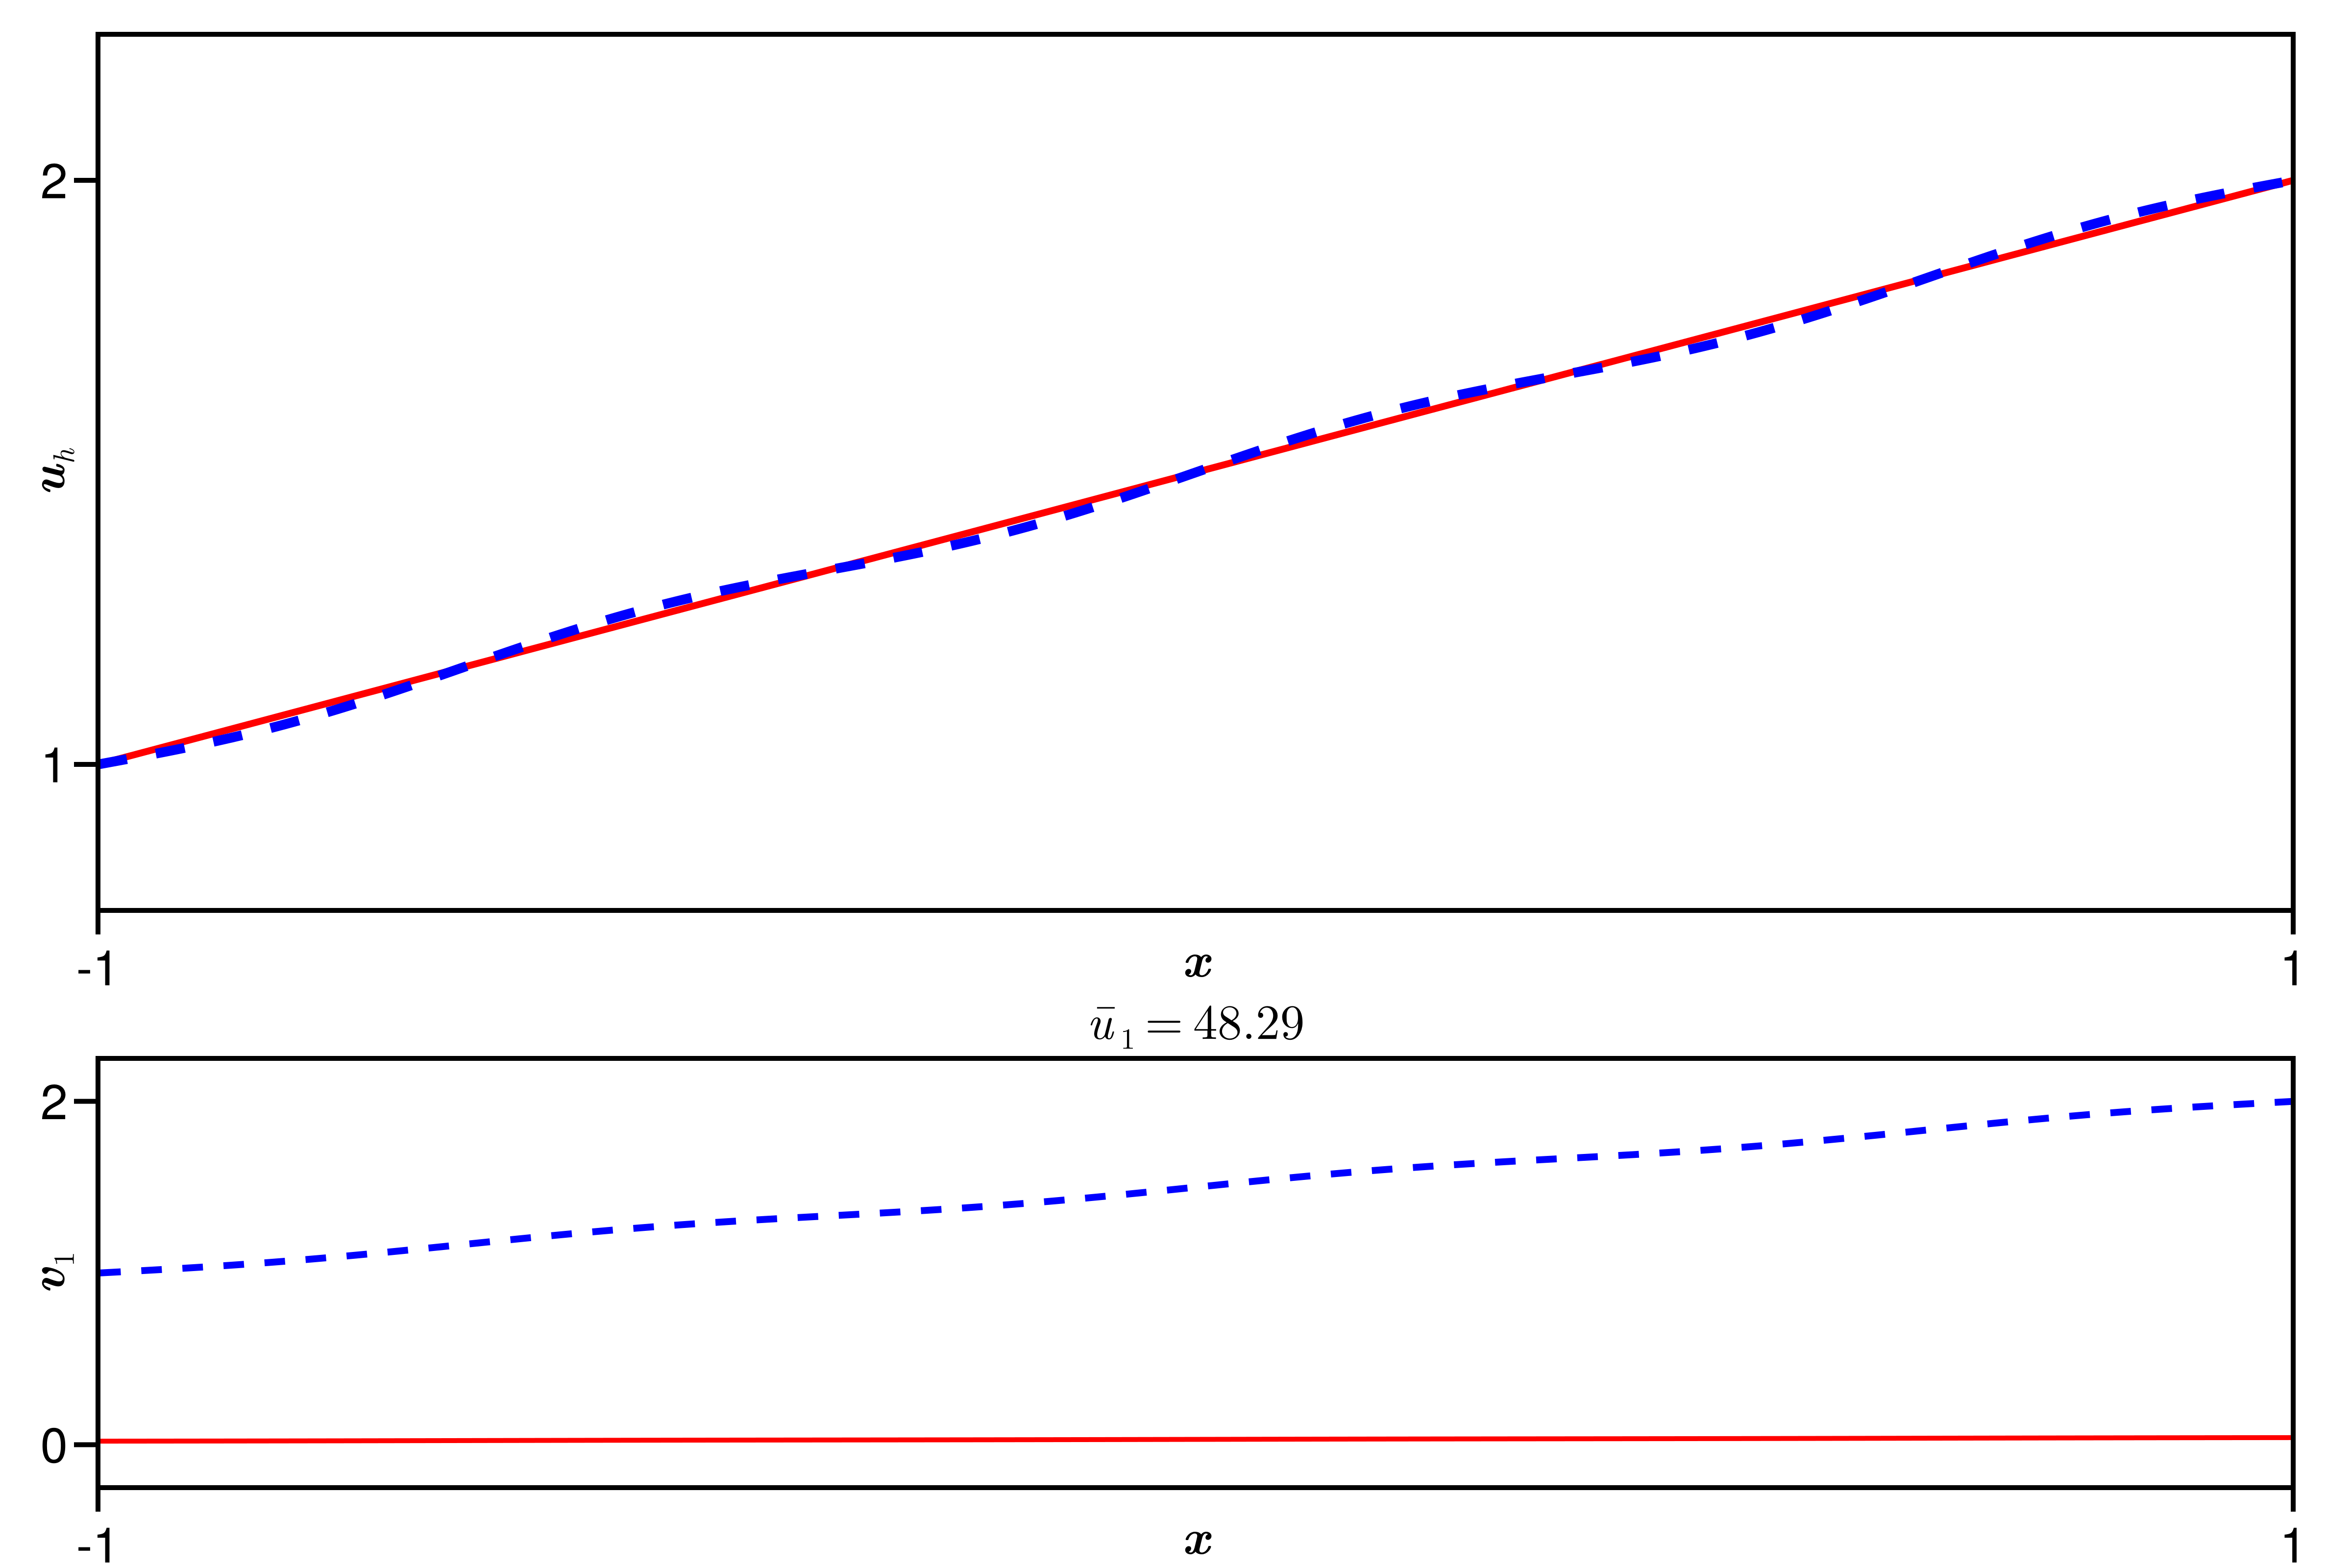
\includegraphics[keepaspectratio, width=0.75\textwidth]{../figures/fig:problem1_rom.png}
    \caption{\textbf{Top}: comparison between the steady-state, time-asymptotic FOM solution (dashed, red) and the reduced-order (dashed, blue) approximation at parameter value $\mu=0.11$.
    \textbf{Bottom}: First singular vector (solid,red) and its weighted representation (dashed, blue) based on the solution $\bar{u}_{1}$ of the ROM (reported at the top).}
    \label{fig:problem1_rom}
\end{figure}

As it can be evinced from Figure \ref{fig:problem1_rom}, although the ROM solution appears less accurate than the elliptic case, it requires only one basis function as $99\%$ of the ``\textit{energy}'' is retained in the first singular value (see Figure \ref{fig:problem1_decay})

\begin{figure}[H]
    \centering 
    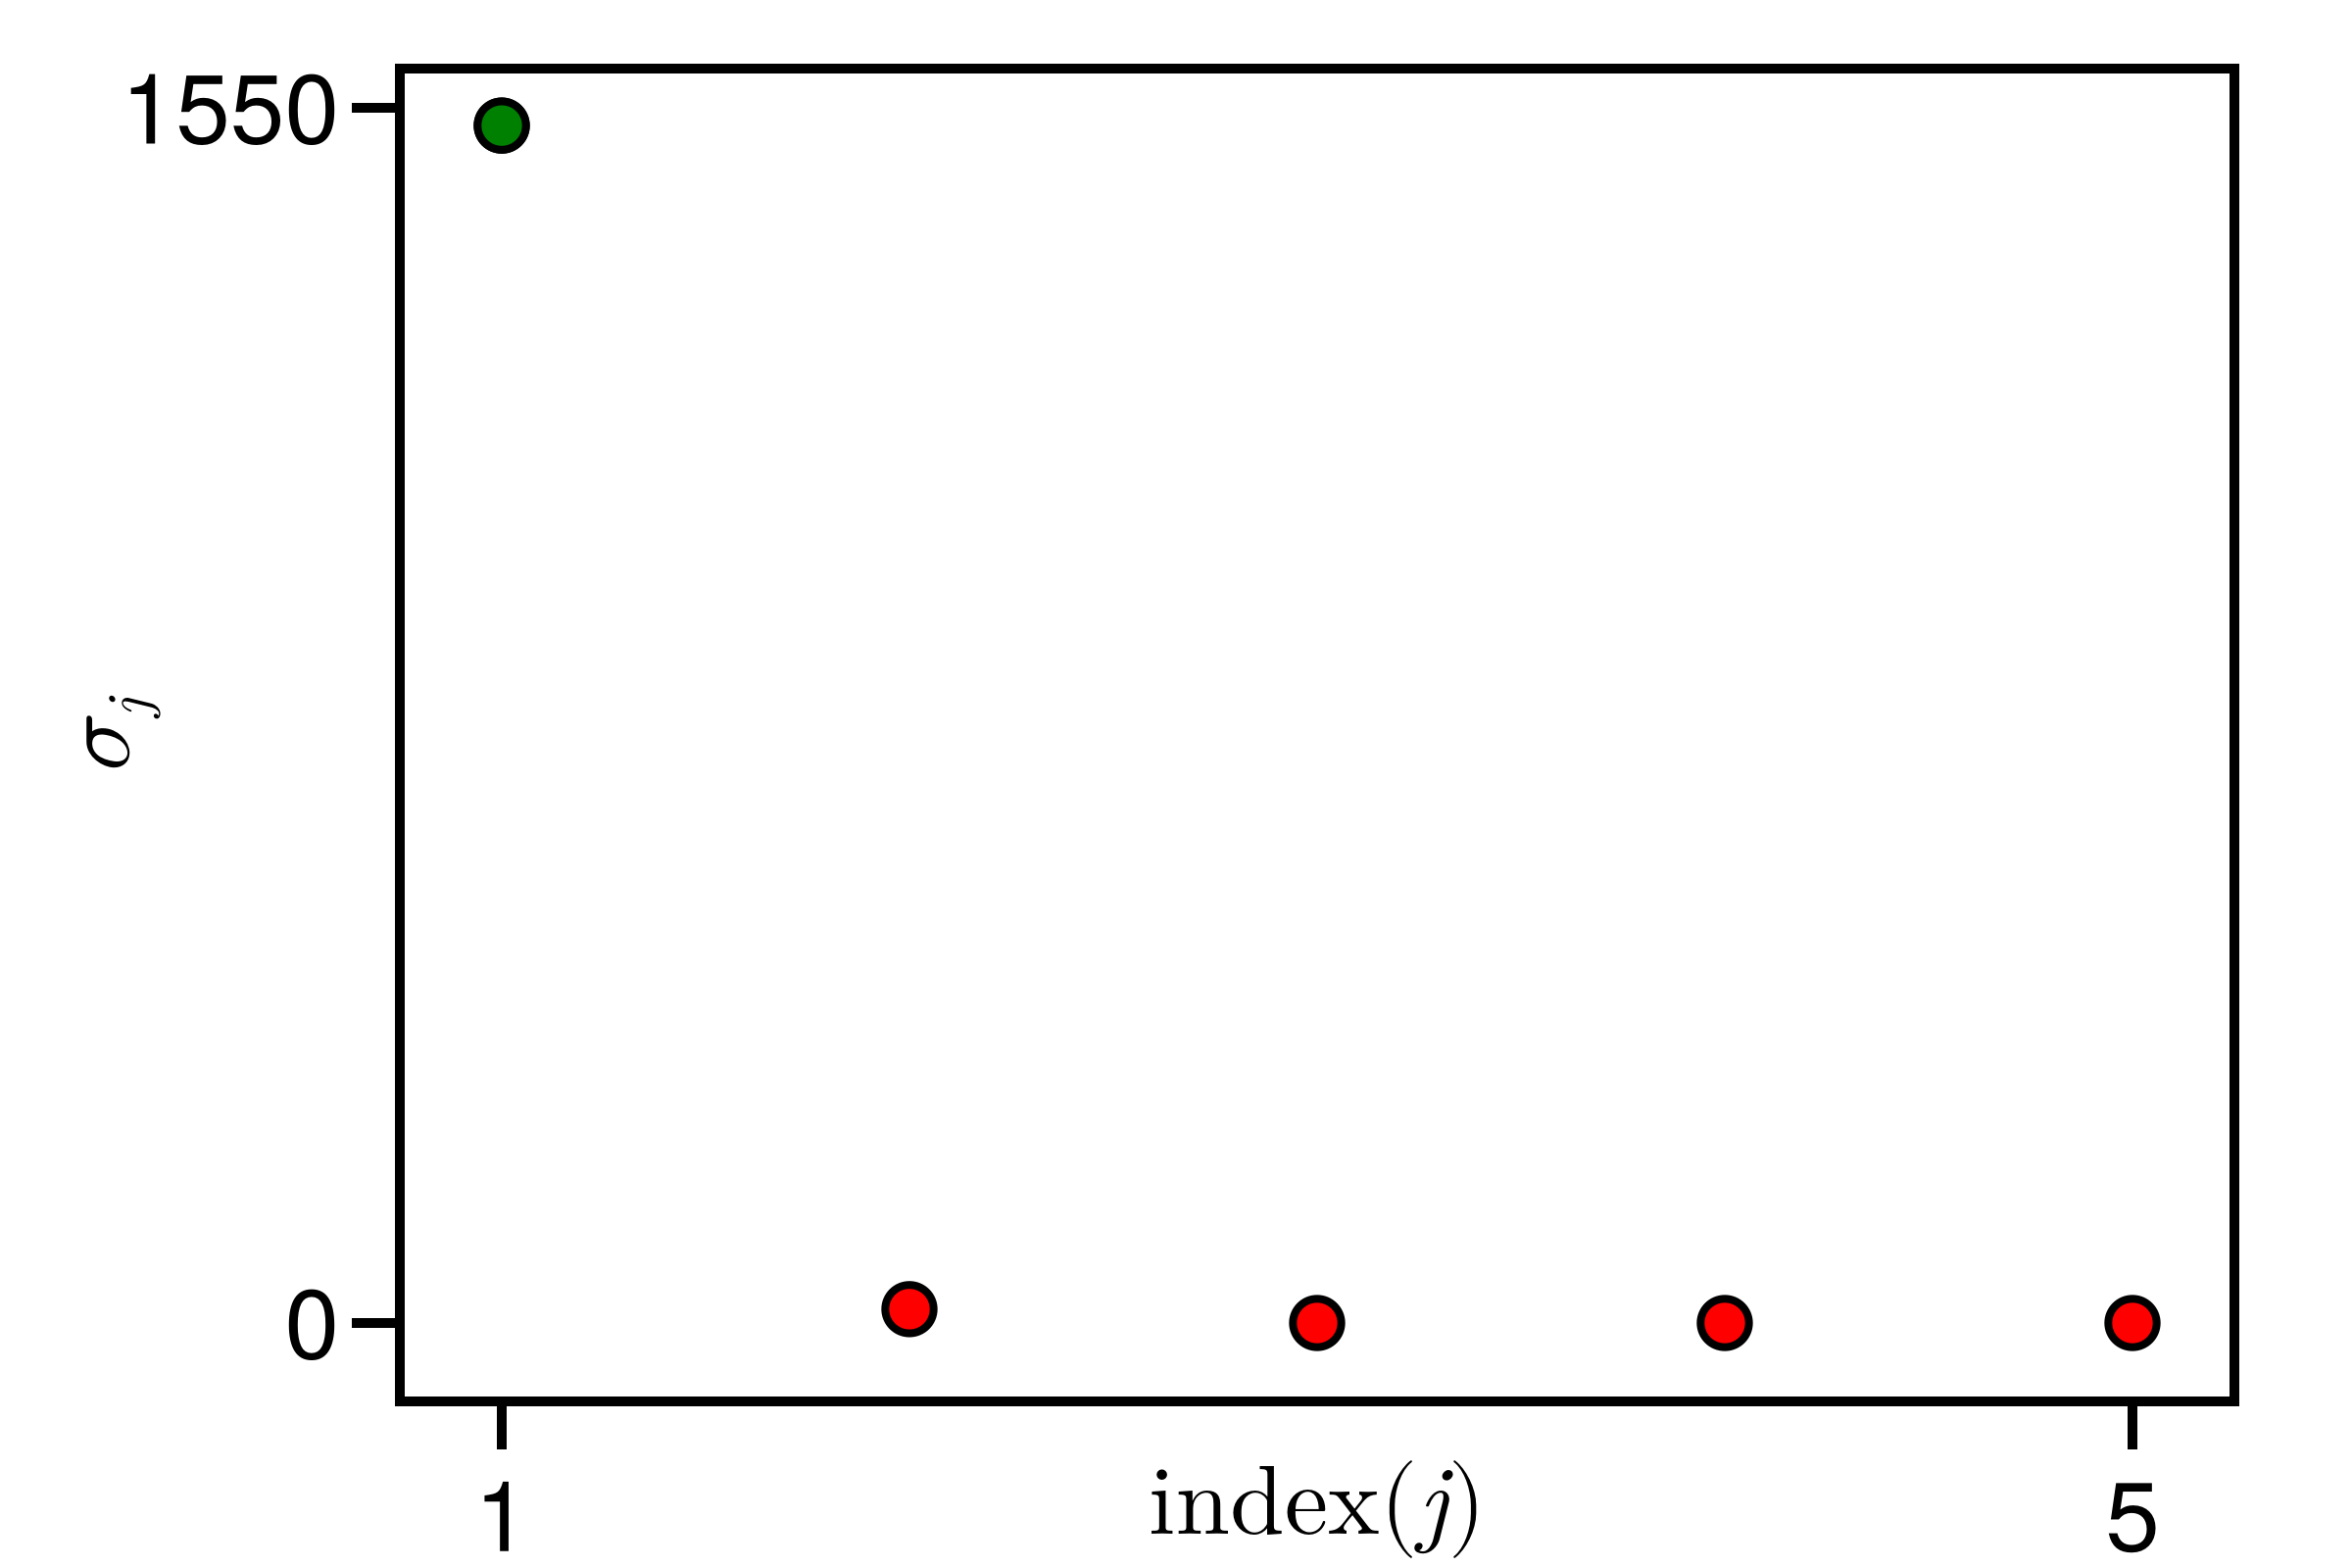
\includegraphics[keepaspectratio, width=0.7\textwidth]{../figures/fig:problem1_decay.png}
    \caption{Kolmogoroff $n-$width decay of problem $1.$ of \eqref{eq:heat}. Green dots reppresent the $N_{r}=1$ singular values used for constructing the ROM.}
    \label{fig:problem1_decay}
\end{figure}

\end{document}
